\documentclass[12pt]{article}
	\usepackage[english]{babel}
	\usepackage[utf8x]{inputenc}
	\usepackage{amsmath}
	\usepackage{graphicx}
	\usepackage[colorinlistoftodos]{todonotes}
	
	\begin{document}
	
	\begin{titlepage}
	
	\newcommand{\HRule}{\rule{\linewidth}{0.5mm}} % Defines a new command for the horizontal lines, change thickness here
	
	\center % Center everything on the page
	 
	%----------------------------------------------------------------------------------------
	%	HEADING SECTIONS
	%----------------------------------------------------------------------------------------
	
	\textsc{\LARGE Testing Policy}\\[0.5cm] % Name of your university/college
	\textsc{\Large Team Hackermen}\\[0.5cm] % Major heading such as course name
	
	
	%----------------------------------------------------------------------------------------
	%	TITLE SECTION
	%----------------------------------------------------------------------------------------
	
	\HRule \\[0.4cm]
	{ \huge \bfseries TicketSalad}\\[0.4cm] % Title of your document
	\HRule \\[1.5cm]
	 
	%----------------------------------------------------------------------------------------
	%	AUTHOR SECTION
	%----------------------------------------------------------------------------------------
	
	\begin{minipage}{0.4\textwidth}
	\begin{flushleft} \large
	\emph{Team Members:}\\% Your name
	Thato \textsc{Mothusi}\\
	Jarryd \textsc{Baillie}\\
	Brandon \textsc{Texeira}\\
	Thomas \textsc{Honiball}\\
	Tristan \textsc{Joseph}\\
	\end{flushleft}
	\end{minipage}
	~
	\begin{minipage}{0.4\textwidth}
	\begin{flushright} \large
	\emph{Client:} \\
	Tribus Digita % Supervisor's Name
	\end{flushright}
	\end{minipage}\\[2cm]
	
	% If you don't want a supervisor, uncomment the two lines below and remove the section above
	%\Large \emph{Author:}\\
	%John \textsc{Smith}\\[3cm] % Your name
	
	
	%----------------------------------------------------------------------------------------
	%	LOGO SECTION
	%----------------------------------------------------------------------------------------
	
	
\includegraphics{ticketSaladLogo.png}\\[1cm] % Include a department/university logo - this will require the graphicx package
	 
	%----------------------------------------------------------------------------------------
	
	\vfill % Fill the rest of the page with whitespace
	
	\end{titlepage}
	
	\section{Testing Processes}
	Since we are adopting scrum methodology and it does not say much about the testing process, we decided to adopt a waterfall approach within our sprint.Our sprints usually last 2 weeks and within those two weeks we develop certain features of the system and once those features are completed, we then write tests for those features we developed. So we are essentially using a white-box testing method whereby we first write code for the system and then write the test cases once we have knowledge of the source code.
	
	\subsection{Functional Requirements Tested}
	\begin{itemize}
		\item A user is able to login
		\item A user is able to claim on an event
		\item A user is able to view their profile
		\item A user is able to add a credit card
		\item A user is able to buy credits
	\end{itemize}
	
	\subsection{Non-Functional Requirements Tested}
	\begin{itemize}
		\item The users password is encrypted
		\item The system is able to handle a minimum of 3000 function calls per second
		\item The system prevents users from entering invalid credit card data
		\item The system prevents proceeding with an incorrect username and/or password
		\item The system database listens on a non-default port
		\item The MongoDB HTTP status interface is not visible on port 28017
		\item The system is using up to date versions of its software
		\item The system uses TLS/SSL encryption for database communication
		\item The system is protected from the following MongoDB vulnerabilities:
			\begin{itemize}
				\item CVE-2015-7882
				\item CVE-2015-2705
				\item CVE-2014-8964
				\item CVE-2015-1609
				\item CVE-2014-3971
				\item CVE-2014-2917
				\item CVE-2013-4650
				\item CVE-2013-3969
				\item CVE-2012-6619
				\item CVE-2013-1892
				\item CVE-2013-2132
			\end{itemize}
	\end{itemize}
	
	\section{Testing Tools}
	Nightwatch is an automated testing framework for web applications and websites, written in Node.js and using the W3C Web-driver API (formerly Selenium Web-driver).Nightwatch relies on "nightwatch.json" as the configuration file to run test files, this json file is placed on the project's root directory. The json file allows for the specification of configuration settings like test environments, test file paths, and selenium specific settings.The reason we chose to use nightwatch is beacuse it has a simple but powerful syntax which enables us to write tests very quickly, using languages like javascript and CSS or Xpath selectors. It also has a built in command-line test runner which can run tests either sequentially or in parallel. Lastly nightwatch allows for flexibility, what this means is that there is a flexible command and assertion framework which makes it easy to extend to implement our application specific commands and assertions.
	
	The Grinder is an application which allows us to write scripts that will test websocket and functional response of the server under a heavy load. We chose to use this application as it was not only able to interface with Meteor functions specifically, but also due to the versatility offered by its code based testing method.
	
	Mongoaudit is an application which runs automated testing to determine vulnerabilities present within our database server. The system provides good insight into what vulnerabilities might be present within our system so that we may take precautions to prevent various attacks such as data injections and side channel attacks targeted at our server.
	
	
	\section{Test Cases}
	Our test cases are located on the master branch in a folder called Testing.Below is a tree structure of where our test cases are located on git.
	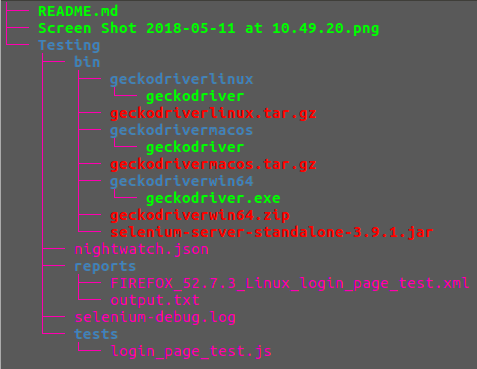
\includegraphics[width=0.8\linewidth, height=8cm]{tree.png}
	
	\section{History}
	
	
	
	
	
	
	
	
	
	\end{document}
	